\documentclass{standalone}
\usepackage{tikz}
\usepackage{pgfplots}
\begin{document}
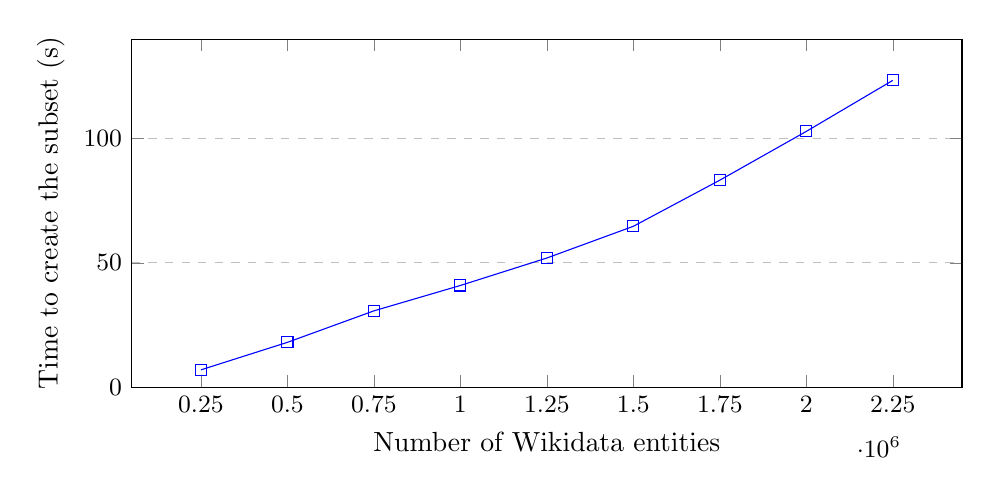
\begin{tikzpicture}
    \begin{axis}[
            title={},
            xlabel={Number of Wikidata entities},
            ylabel={Time to create the subset (s)},
            ymin=0, ymax=140,
            xtick=data,
            height=6cm,
            width=\textwidth,
            legend pos=north west,
            ymajorgrids=true,
            grid style=dashed,
            tick align=inside,
            every tick label/.append style={font=\small}
        ]
        \addplot[
            color=blue,
            mark=square,
        ]
        coordinates {
                (250000,6.962351676)
                (500000,18.032416884)
                (750000,30.703393638)
                (1000000,40.914275035)
                (1250000,51.969880152)
                (1500000,64.728383731)
                (1750000,83.286143031)
                (2000000,102.919394550)
                (2250000,123.450540619)
            };
    \end{axis}
\end{tikzpicture}
\end{document}